
\section{Принцип максимума для параболического уравнения.}
%Никитушка отмочил красоту
$\bullet$ Пусть $\Omega$ -- ограниченная область в $\R^n$, $T > 0$, 
$Q_T = (0,T) \times \Omega$ - цилиндр. Сечение цилиндра плоскостью $t = \tau$ обозначим $\Omega_\tau$.

\begin{definition}
{\bf Параболическая граница области $Q_T$} -- множество $\Gamma_T = \Omega_0 \cup \{[0,T] \times \partial{\Omega} \}$.
\end{definition}
\begin{center}
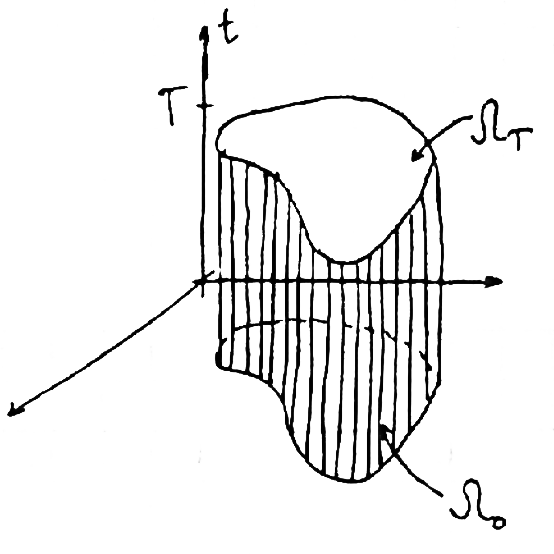
\includegraphics[scale=0.5]{13_1_new}
\end{center}

Определим оператор $\mathrm{L} : \mathrm{L}u(t,x) = u_t - a^2 \Delta_xu$, где 
$u \in C_{t, x}^{1,2}(Q_T)$.

\begin{theorem}[Принцип максимума]
Пусть $u(t,x) \in C_{t, x}^{1,2}(Q_T) \cap C(\overline{Q_T})$, и пусть 
$\mathrm{L}u(t,x) \leq 0$ в $Q_T$. Тогда $\max\limits_{(x,t) \in \overline{Q_T}} u(t,x)$ достигается на параболической границе $ \Gamma_T $ области $Q_T$.


\begin{proof}
Возьмем усеченный цилиндр $Q_{T-\delta}$. Рассматриваются $M = \max\limits_{\overline{Q_{T-\delta}}} u(t,x)$ и $m = \max\limits_{\Gamma_{T-\delta}} u(t,x)$. Теорема утверждает, что $M$ не превосходит $m$.\\
\begin{itemize}
\item {\bf Пусть это не так} и $m < M$. Тогда $\exists (t^1,x^1) \in Q_{T-\delta} \cup \Omega_{T-\delta}$ такая, что $M = u(t^1, x^1)$. \\
Т.к. это точка максимума гладкой функции, $u_{x_ix_i}(t^1,x^1) \leq 0$, а $u_t(t^1, x^1) \geq 0$ (Если внутри, то равенство, если на верхней кромке, то $\geq 0$).\\
Значит, значение образа $u(t,x)$ под действием оператора $\mathrm{L}$ в точке $(t^1, x^1): \boxed{\mathrm{L}u(t^1, x^1) = \eval{(u_t -a^2 \Delta_x u)}_{(t^1,x^1)}  \geq 0}$.\\
Для противоречия необходимо показать, что неравенство строгое.\\

 \item {\bf Строгость:}
Возьмем функцию $v_\beta(t,x) = u(t,x) +\beta \abs*{x-x^1}^2, \, \beta = \dfrac{M-m}{2(\mathrm{diam} \, Q_T)^2}$ -- такая же гладкая, как $u$.\\
 На параболической границе $v_\beta \leq m + \frac{M-m}{2d^2}\cdot d^2 = \frac{M+m}{2} < M$.
Тем не менее, $v_\beta(t^1, x^1) = M \Rightarrow$ максимум $v_\beta$ не на параболической границе.\\
Пусть он в точке $(t^2, x^2) \notin \Gamma_{T-\delta}$. Тогда $\mathrm{L}\eval*{v_\beta}_{(t^2,x^2)} = \mathrm{L}\eval{u}_{(t_2, x_2)} - a^2 \beta 2n \boxed{\geqslant} 0 \Rightarrow \\
\mathrm{L}\eval{u}_{(t_2,x_2)} \geq a^2 \beta 2n > 0 \Rightarrow$
{\bf Противорчие} (вывод $\boxed{\geq}$ аналогичен рамке выше)
 
\item {\bf Предельный переход с $\delta \rightarrow+0$:}
Пусть $u_{*} = \max\limits_{\Gamma_T} u(t,x)$. \\
Тогда $\max\limits_{\overline{Q_{T-\delta}}}u(t,x) \leq \max\limits_{{\Gamma_{T-\delta}}}u(t,x) \leq \max\limits_{{\Gamma_{T}}}u(t,x) = u_* \Rightarrow
u(t,x) \leq u_*$
во всех точках $\overline{Q_T} \backslash \Omega_T$.\\
$\eval{u(t,x)}_{\Omega_T} = \lim\limits_{(\widehat{t}, \widehat{x}) \in Q_T \rightarrow (t,x) \in \Omega_T} u(\widehat{t},\widehat{x}) \boxed{\leq} u_*$ 
\\($\boxed{\leq}$ - предельный переход в неравенствах.) Теорема доказана.
\end{itemize}

\end{proof}
\end{theorem}


\begin{conseq}
Пусть $u(t,x) \in C^{1,2}_{t,x}(Q_T) \cap C(\overline{Q_T}), \mathrm{L}u = 0 \Forall(t,x) \in Q_T$.
 Тогда $\max\limits_{\overline{Q_T}}u(t,x)$ и $\min\limits_{\overline{Q_T}}u(t,x)$ достигаются на параболической границе $\Gamma_T$ множества $Q_T$.
 \begin{proof}
 Максимум достигается, т.к. $\mathrm{L}u \leq 0$, минимум достигается, т.к. $\mathrm{L}(-u) \leq 0$.
 \end{proof}
\end{conseq}
